\documentclass{birkmult}

\usepackage[utf8]{inputenc}

\usepackage{url}
\usepackage{hyperref}
\usepackage[hyphenbreaks]{breakurl}

\usepackage{commands}

 \newtheorem{thm}{Theorem}[section]
 \newtheorem{cor}[thm]{Corollary}
 \newtheorem{lem}[thm]{Lemma}
 \newtheorem{prop}[thm]{Proposition}
 \theoremstyle{definition}
 \newtheorem{defn}[thm]{Definition}
 \theoremstyle{remark}
 \newtheorem{rem}[thm]{Remark}
 \newtheorem*{ex}{Example}
 \numberwithin{equation}{section}

\def\HOML{\entity{HOML}\xspace}
\def\HOL{\entity{HOL}\xspace}


\begin{document}

%-------------------------------------------------------------------------
% editorial commands: to be inserted by the editorial office
%
%\firstpage{1} \volume{228} \Copyrightyear{2004} \DOI{003-0001}
%
%
%\seriesextra{Just an add-on}
%\seriesextraline{This is the Concrete Title of this Book\br H.E. R and S.T.C. W, Eds.}
%
% for journals:
%
%\firstpage{1}
%\issuenumber{1}
%\Volumeandyear{1 (2004)}
%\Copyrightyear{2004}
%\DOI{003-xxxx-y}
%\Signet
%\commby{inhouse}
%\submitted{March 14, 2003}
%\received{March 16, 2000}
%\revised{June 1, 2000}
%\accepted{July 22, 2000}
%
%
%
%---------------------------------------------------------------------------
%Insert here the title, affiliations and abstract:
%


\title[Modal Collapse]
 {The Ontological Modal Collapse \\ 
 as a Collapse of the Square of Opposition}


\author[Benzm\"uller]{Christoph Benzm\"uller}

\address{%
Department of Mathematics and Computer Science\\
Arnimallee 7 \\
Room 115 \\
14195 Berlin \\
Germany
}

\email{c.benzmueller@gmail.com}


\author[Woltzenlogel-Paleo]{Bruno Woltzenlogel Paleo}
\address{ 
Favoritenstra{\ss}e 9 \\
Room HA0402 \\
1040 Wien \\
Austria
}
\email{bruno.wp@gmail.com}




%----------classification, keywords, date
\subjclass{
Prim. 03A02;  % Philosophical aspects of logic and foundations
Sec. 68T02 % Artificial Intelligence
\marginpar{Change?: 03B15, 03B45, 03B35, 68T15}
}

\keywords{Modal Logics, Higher-Order Logics, Ontological Argument,
  Interactive and Automated Theorem Proving}

\date{August 30, 2014}

\dedicatory{ }


\begin{abstract}
The \emph{modal collapse} that afflicts G\"odel's modal ontological 
argument for God's existence is discussed from the perspective of the 
modal square of opposition.
\end{abstract}


\maketitle

%\tableofcontents

\section{Introduction}

Attempts to prove the
existence (or non-existence) of God by means of abstract, ontological
arguments are an old tradition in western philosophy, with contributions by several prominent philosophers, including St. Anselm of
Canterbury, Descartes and Leibniz. Kurt G{\"o}del and Dana Scott studied and further improved this argument, bringing it to a mathematically more precise form, as a chain of axioms, lemmas and theorems in a second-order modal logic \cite{GoedelNotes,ScottNotes}, shown in Fig. \ref{fig:scott}.

\begin{figure}[t]
\noindent \framebox[\columnwidth][r]{
\begin{minipage}{.94\columnwidth}\small
\begin{itemize}
\item[\textbf{A1}] Either a property or its negation is positive, but not
  both:
  $$\hol{\allq \varphi [P(\neg \varphi) \biimp \neg P(\varphi)]}$$ 
\item[\textbf{A2}] A property necessarily implied by a
  positive property is positive:
  $$\hol{\allq \varphi \allq \psi [(P(\varphi) \wedge \nec \allq x [\varphi(x)
  \imp \psi(x)]) \imp P(\psi)]}$$
\item[\textbf{T1}] Positive properties are possibly exemplified: 
  $$\hol{\allq \varphi [P(\varphi) \imp \pos \exq x \varphi(x)]}$$ 
\item[\textbf{D1}] A \emph{God-like} being possesses all positive properties: 
  $$\hol{G(x) \equiv \forall \varphi [P(\varphi) \imp \varphi(x)]}$$ 
\item[\textbf{A3}]  The property of being God-like is positive: 
  $$\hol{P(G)}$$
\item[\textbf{C\phantom{1}}] Possibly, a God-like being exists: $$\hol{\pos \exq x G(x)}$$
\item[\textbf{A4}]  Positive properties are necessarily positive: 
  $$\hol{\allq \varphi [P(\varphi) \imp \Box \; P(\varphi)]}$$ 
\item[\textbf{D2}] An \emph{essence} of an individual is a property possessed by it and necessarily implying any of its properties: $$\hol{\ess{\varphi}{x} \equiv \varphi(x) \wedge \allq
  \psi (\psi(x) \imp \nec \allq y (\varphi(y) \imp \psi(y)))}$$ 
\item[\textbf{T2}]  Being God-like is an essence of any
  God-like being: $$\hol{\allq x [G(x) \imp \ess{G}{x}]}$$
\item[\textbf{D3}] \emph{Necessary existence} of an individual is the necessary exemplification of all its essences: 
  $$\hol{\NE(x) \equiv \allq \varphi [\ess{\varphi}{x} \imp \nec
  \exq y \varphi(y)]}$$
\item[\textbf{A5}] Necessary existence is a positive property: $$\hol{P(\NE)}$$ 
\item[\textbf{L1}] If a god-like being exists, then necessarily a god-like being exists: 
  $$\hol{\exq x G(x) \imp \nec \exq y G(y)}$$
\item[\textbf{L2}] If possibly a god-like being exists, then necessarily a god-like being exists: 
  $$\hol{\pos \exq x G(x) \imp \nec \exq y G(y)} $$
%
\item[\textbf{T3}] Necessarily, a God-like being exists: $$\hol{\nec \exq x G(x)}$$ 
\end{itemize}
\end{minipage}
} \vskip-.5em
\caption{Scott's version of G\"odel's ontological argument \cite{ScottNotes}.\label{fig:scott}} 
\end{figure}

G\"{o}del defines God as a being who possesses all \emph{positive}
properties and states a few reasonable (but debatable) axioms that
such properties should satisfy.  
The overall idea of G{\"o}del's proof
is in the tradition of Anselm's argument, who defined God as some
entity of which nothing greater can be conceived. 
Anselm argued that
existence in the actual world would make 
such an assumed being even
greater (more perfect); 
hence, by definition, God must exist. However,
for Anselm existence was treated as a predicate and 
the possibility of God's existence was assumed as granted. 
These issues were criticized by Kant and Leibniz, 
respectively, and they were addressed in the work of G\"odel.

Nevertheless, G{\"o}del's work still leaves room for criticism.  In
particular, his axioms are so strong that, when assuming unrestricted
comprehension principles\footnote{A possible direction to remedy modal
  collapse, as studied e.g. by Koons
  \cite{koons06:_sobel_goedel_ontol_proof} is to impose restrictions
  on the domain of properties.}, 
\marginpar{added footnote}
they entail a \emph{modal collapse}
\cite{Sobel1987,sobel2004logic}: everything that is the case is so
necessarily.  There has been an impressive body of recent and ongoing
work
(cf.~\cite{sobel2004logic,Fitting,anderson90:_some_emend_of_goedel_ontol_proof,AndersonGettings,bjordal99,fuhrmann05:_exist_notwen,Hajek2002,Hajek2008,ContemporaryBibliography}
and the references therein) proposing solutions for the modal
collapse.  The goal of this contribution is to discuss the modal
collapse from the point of view of the modal square of opposition.
\marginpar{@Bruno: Shall we add a sentence or two here?} 


\section{A Collapse of the Modal Square}

A crucial step of most ontological arguments is the claim that if
God's existence is possible, then it is necessary.  This is Lemma
\textbf{L2} in G\"odel's proof.  In the modal square of opposition
(Fig. \ref{fig:square}), this is an unusual situation in which the
\textbf{I} corner must imply and entail the \textbf{A} corner, 
in the particular case when $\phi$ is $\exq x G(x)$.  
G\"odel's proof shows that his axioms are indeed 
strong enough to invert the direction of
entailment for this choice of $\phi$.  
This observation, however, immediately leads 
to the question whether the axioms are eventually 
even strong enough to enable the inverted entailment
for any arbitrary sentence $\phi$.  
That is essentially the question asked by 
Sobel \cite{Sobel1987}, and his proof of the modal collapse
(\textbf{MC}, cf. Fig.~\ref{fig:collapse}) 
provides an affirmative answer. It is possible to show
that this form of the modal collapse entails (in modal logic
\textbf{\emph{K}}) a collapse of the modal square (\textbf{MCs}),
causing the subcontraries to entail 
(and even imply) their respective
contraries. Normally, as shown in Fig. \ref{fig:square}, 
in the modal square of opposition only the 
other direction of entailment holds: the
contraries entail their subcontraries, 
assuming the \emph{modal existential import} \textbf{ExImp}
\cite{ExImport}.

Moreover, in any modal logic where the axiom \textbf{T} holds
(i.e. where the accessibility relation is reflexive), 
even a total collapse of the modalities (\textbf{MCt}) 
is entailed by \textbf{MC}.
Interestingly, under this stronger form of modal
collapse, the contraries entail their subcontraries even 
without the existential import.

\begin{figure}[t]
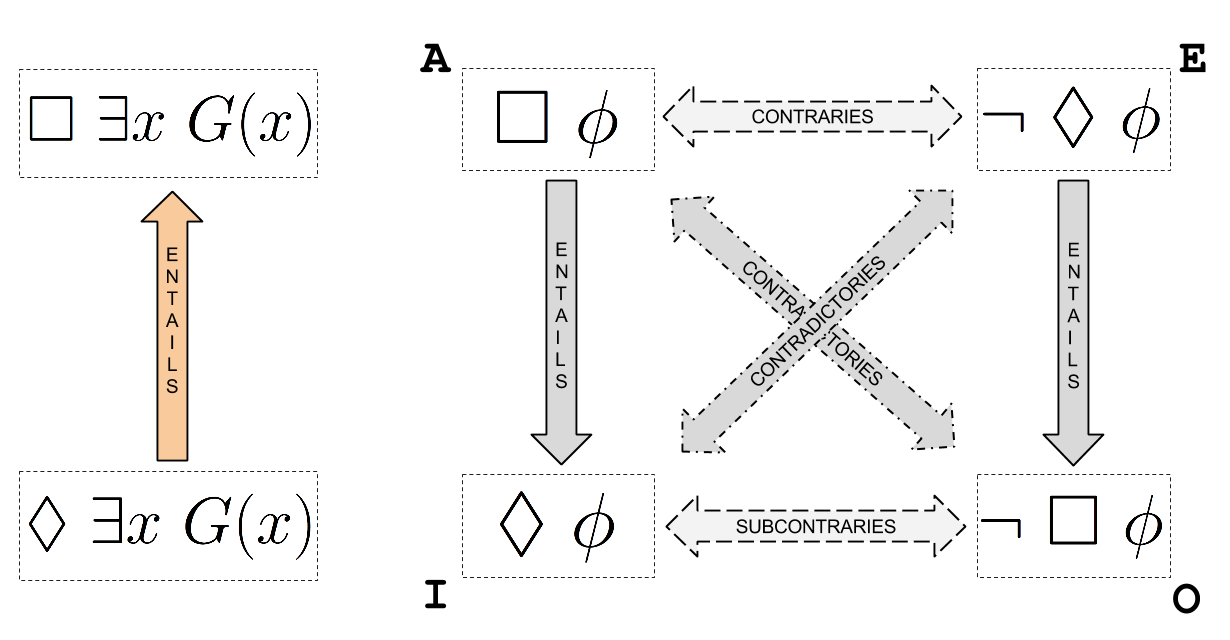
\includegraphics[width=0.9\textwidth]{SquarePics/ModalSquare.png}
\caption{Modal Square of Opposition.}
\label{fig:square}
\end{figure}



\begin{figure}[t]
\noindent \framebox[\columnwidth][r]{
\begin{minipage}{.94\columnwidth}\small
\begin{itemize}
\item[\textbf{MC}] Everything that is the case is so necessarily:
  $\hol{\allq \phi [\phi \imp \nec \phi]}$ \\
\item[\textbf{MCs}] Everything that is possible is necessary:
  $\hol{\allq \phi [\pos \phi \imp \nec \phi]}$  \\
\item[\textbf{T}] Everything that is necessary is the case:
  $\hol{\allq \phi [\nec \phi \imp \phi]}$ \\
\item[\textbf{ExImp}] (Modal Existential Import):
  $\hol{\pos \top}$ \\
\item[\textbf{AI}] Everything that is necessary is possible:
  $\hol{\allq \phi [\nec \phi \imp \pos \phi]}$ \\
\item[\textbf{MCt}] Modalities collapse completely:
  $\hol{\allq \phi [(\phi \biimp \nec \phi) \wedge (\pos \phi \biimp \nec \phi)]}$
\end{itemize}
\end{minipage}
} \vskip-.5em
\caption{Modal Collapse}
\label{fig:collapse} 
\end{figure}

\newcommand{\collapse}[1]{\mathit{collapse}(#1)}

Although G\"odel's axioms lead to modal collapse, 
there are several variants 
(e.g. \cite{anderson90:_some_emend_of_goedel_ontol_proof,AndersonGettings,bjordal99}) 
that are known to be immune to it. 
This means there must be at least one proposition $\phi$ 
such that the implication $\phi \imp \nec \phi$ 
(from now on abbreviated as $\collapse{\phi}$) is not valid 
under the axioms and definitions used by the variant. 
But if the variant is sufficiently similar to G\"odel's argument, 
also deriving Lemmas \textbf{L1} and 
\textbf{L2}, then 
$\collapse{\exq x G(x)}$ must be valid. 
Therefore, one may wonder how strong is their immunity to 
the modal collapse: is there any other proposition $\phi$ 
for which $\collapse{\phi}$ is also valid?

For Anderson's emendation 
\cite{anderson90:_some_emend_of_goedel_ontol_proof}, 
for example, a form of the modal collapse (\textbf{A:MC}), 
restricted to positive properties applied to god-like beings, 
can be derived. The proof, under the modal logic 
\textbf{\emph{K}}, depends only on Anderson's 
alternative definition of god-like being (\textbf{A:D1}). 
This class of propositions for which the collapse occurs 
is tight: weaker restrictions 
(\textbf{A:MC1} and \textbf{A:MC2}), 
which could lead to larger classes, are counter-satisfiable. 
These results hold under both constant and varying domain 
quantification, with possibilist and actualist quantifiers.


\begin{figure}[t]
\noindent \framebox[\columnwidth][r]{
\begin{minipage}{.94\columnwidth}\small
\begin{itemize}
\item[\textbf{A:D1}] A \emph{God-like} being necessarily possesses those and only those properties that are positive: 
  $$\hol{G_A(x) \equiv \forall \varphi [P(\varphi) \biimp \nec \varphi(x)]}$$ 
\item[\textbf{A:MC}] The modal collapse happens for any positive properties applied to any god-like being:
  $$
  \hol{\allq \varphi \allq x [(P(\varphi) \wedge G_A(x)) \imp \collapse{\varphi(x)}]}
  $$
\item[\textbf{A:MC1}] The modal collapse does \emph{not} happen for positive properties applied to arbitrary individuals (\emph{counter-satisfiable}):
  $$
  \hol{\allq \varphi \allq x [P(\varphi) \imp \collapse{\varphi(x)}]}
  $$
\item[\textbf{A:MC2}] The modal collapse does \emph{not} happen for an arbitrary properties applied to a god-like being (\emph{counter-satisfiable}):
  $$
  \hol{\allq \varphi \allq x [G_A(x) \imp \collapse{\varphi(x)}]}
  $$
\end{itemize}
\end{minipage}
} \vskip-.5em
\caption{Restricted Collapse for Anderson's Emendation \cite{anderson90:_some_emend_of_goedel_ontol_proof}}
\label{fig:anderson}
\end{figure}


Independently of the variant of the ontological argument 
under consideration, the following can be said about 
classes of collapsing propositions:
\begin{enumerate}
\item Valid propositions are collapsing: 
if $\phi$ is valid, then $\collapse{\phi}$ is valid.
%
\item The class of collapsing propositions 
is closed under logical equivalence: 
if $\collapse{\phi}$ is valid and $\phi \biimp \phi'$ is valid, 
then $\collapse{\phi'}$ is valid.
%
\item The class of collapsing propositions is 
not generally closed under equi-validity: 
even if $\collapse{\phi}$ is valid and $\phi$ and $\phi'$ 
are equi-valid, \\ $\collapse{\phi'}$ may not be valid.
%
\item The class of collapsing propositions is 
not generally closed under implication: 
even if $\collapse{\phi}$ is valid and 
$\phi \imp \phi'$ is valid, 
$\collapse{\phi'}$ may not be valid.
\end{enumerate} \marginpar{@Bruno: Shall we respond here to the
  rewievers criticism?}



\section{Final Remarks}

\sloppy All results announced in this note have been 
obtained experimentally using interactive and 
automated theorem provers and model finders
\cite{LEO,Satallax,Isabelle,Coq,Nitpick}.  
The source codes of the experiments, 
as well as the resulting proofs and counter-models, 
are available in
\url{github.com/FormalTheology/GoedelGod/}
in the files \url{ModalCollapse.thy} and \texttt{ModalSquareOfOpposition.thy} inside the folder \url{Formalizations/Isabelle/Meta} as well as in files inside the folder \texttt{Formalizations/Isabelle/Anderson}.

The technique enabling these experiments is the embedding of 
quantified modal logics into higher-order logics 
\cite{J23,B9,C36}, for which automated theorem provers exist. 
This technique has already been successfully employed in the 
verification and reconstruction of G\"odel's proof 
\cite{J28,J30,W50,J29}, and a detailed 
mathematical description is available in \cite{C40}.

The modal collapse is an interesting example of philosophical 
controversy and dispute, to which we can apply Leibniz's idea 
of a \emph{calculus ratiocinator} brought to reality in the 
form of contemporary automated theorem provers. 
A significant advantage provided by the use of computers is 
that all parameters (e.g. modal logic, domain conditions, 
semantics) under which the announced results hold must be 
explicitly specified in the source code. This reduces the need 
for interpretation and the danger of misunderstandings. 
Current technology is increasingly ready to be embraced by 
those willing to practice computer-assisted theoretical 
philosophy \cite{oppenheimera11,rushby13}.

Ongoing and future work includes the computer-assisted 
study of the modal collapse in
other variants of the ontological argument (e.g.~\cite{bjordal99,fuhrmann05:_exist_notwen}). Furthermore, our experiments in Isabelle revealed a weakness of the current integration of the HOL-ATPs LEO-II and Satallax via Sledgehammer: most of the problems in our study solved by the two HOL-ATPs were still too hard to be reconstructed and verified by Isabelle's internal prover Metis. This points to relevant future work regarding the integration of HOL-ATPs in Isabelle.
 


\subsection*{Acknowledgment}

We would like to thank Paul Weingartner, Andr\'{e} Fuhrmann 
and Melvin Fitting for several discussions about 
G\"odel's ontological argument.


\subsection*{Note about authorship}

Alphabetic order has been used for the authors' names. 
The extent and kind of contribution of each author 
cannot be inferred from the order.

\bibliographystyle{plain}
\bibliography{Bibliography}

\end{document}
